\section{MÔ HÌNH TÌM KIẾM HYBRID}
\subsection{Xử lý dữ liệu}
\begin{figure}[H]
    \centering
    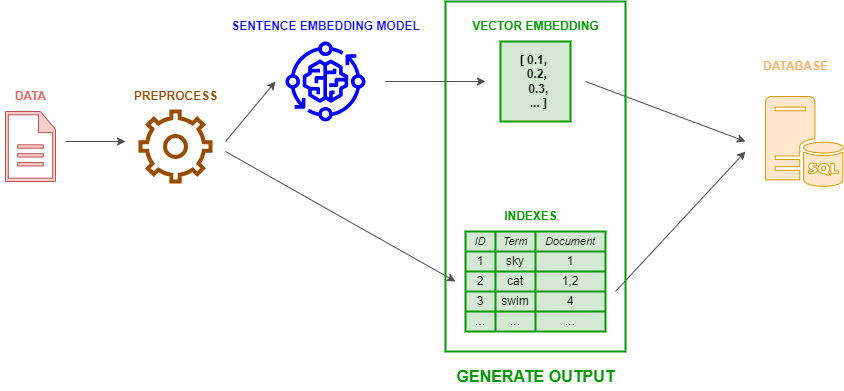
\includegraphics[,width=\textwidth]{Images/HybridSearch/DataProcess.png}
    \caption{Sơ đồ các bước xử lý dữ liệu cho mô hình tìm kiếm Hybrid}
\end{figure}
Quá trình xử lý dữ liệu cho mô hình tìm kiếm bao gồm các bước sau:
\begin{itemize}
    \item Làm sạch dữ liệu:
    \begin{itemize}
        \item Dữ liệu dạng chuỗi (string) được làm sạch để loại bỏ các ký tự đặc biệt, khoảng trắng thừa, và chuẩn hóa văn bản. Quá trình này giúp cải thiện chất lượng và độ chính xác của việc tìm kiếm.
        \item Các bước làm sạch bao gồm: chuyển đổi toàn bộ văn bản về chữ thường, loại bỏ dấu câu, loại bỏ các từ dư thừa hoặc không cần thiết (stop words), và xử lý các lỗi chính tả cơ bản.
    \end{itemize}
    \item Chuyển đổi văn bản thành vector(Embedding):
    \begin{itemize}
        \item Nhóm sử dụng Sentence Transformer để chuyển đổi văn bản đã làm sạch thành các vector số học (embedding). Các vector này biểu thị ý nghĩa ngữ nghĩa của văn bản, giúp hệ thống hiểu được ngữ cảnh và ý định của người dùng.
        \item Quá trình embedding tạo ra các vector có độ chiều cao (high-dimensional vectors), cho phép so sánh và tìm kiếm ngữ nghĩa một cách hiệu quả.
    \end{itemize}
    \item Đánh chỉ mục (Indexing):
    \begin{itemize}
        \item Dữ liệu văn bản sau khi làm sạch cũng được đánh chỉ mục để sử dụng cho việc tìm kiếm toàn văn bản. Việc đánh chỉ mục giúp tăng tốc độ truy vấn, đảm bảo rằng các từ khóa người dùng nhập sẽ được tìm kiếm và so khớp một cách nhanh chóng.
    \end{itemize}
    \item Lưu trữ vào cơ sở dữ liệu:
    \begin{itemize}
        \item Cả vector embedding và chỉ mục của dữ liệu văn bản được lưu trữ trong cơ sở dữ liệu. Điều này giúp hệ thống truy cập và sử dụng thông tin một cách hiệu quả khi thực hiện các truy vấn tìm kiếm.
    \end{itemize}
\end{itemize}
\begin{figure}[H]
    \centering
    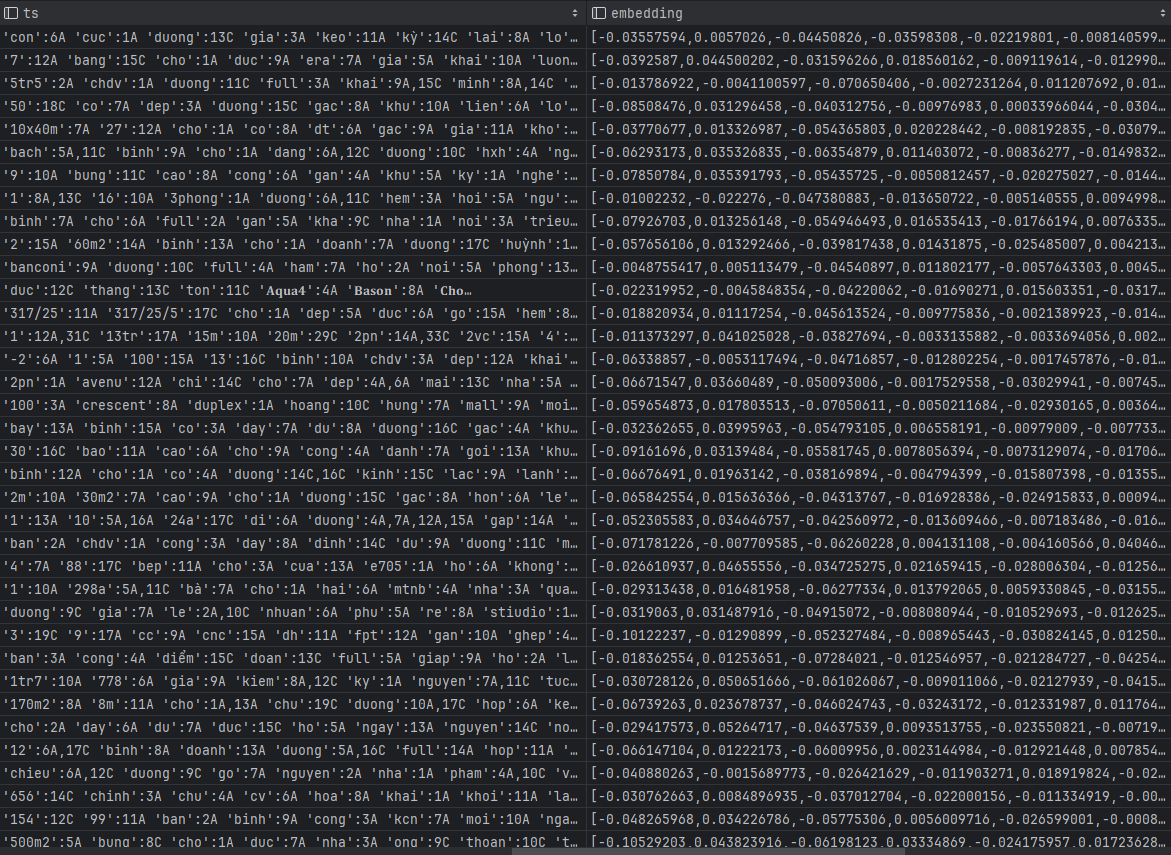
\includegraphics[width=\textwidth]{Images/HybridSearchResult.png}
    \caption{Dữ liệu văn bản sau khi được đánh chỉ mục và chuyển đổi thành dạng vector}
\end{figure}

\subsection{Kiến trúc tìm kiếm với mô hình Hybrid}
Mô hình Hybrid Search kết hợp cả Tìm kiếm toàn văn bản và Tìm kiếm ngữ nghĩa, cùng với cơ chế reranking để tối ưu hóa kết quả tìm kiếm, đảm bảo trải nghiệm tìm kiếm chính xác và hiệu quả cho người dùng. Dưới đây là chi tiết về kiến trúc mô hình:
\begin{figure}[H]
    \centering
    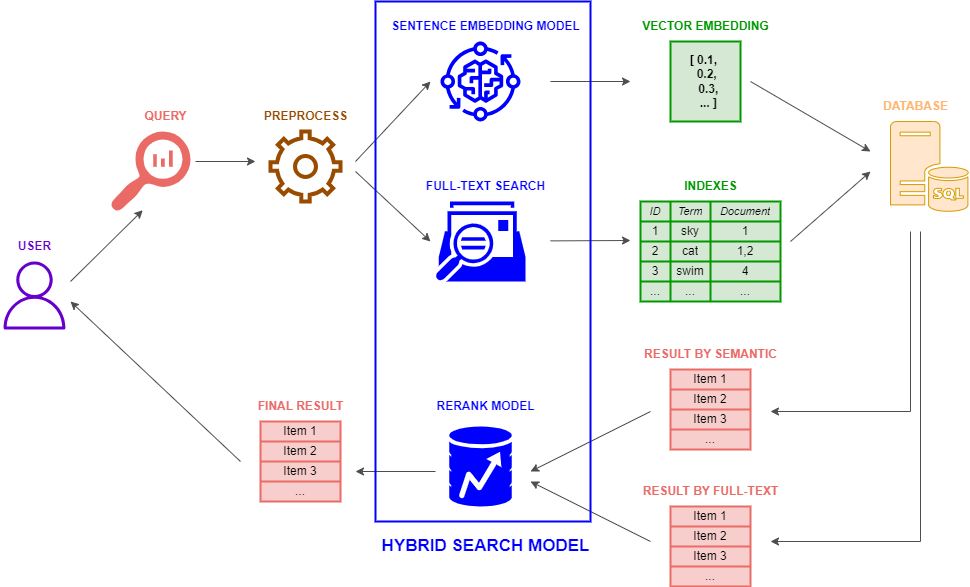
\includegraphics[width=\textwidth]{Images/HybridSearch/SearchArchitecture.png}
    \caption{Sơ đồ kiến trúc của mô hình tìm kiếm Hybrid}
\end{figure}
Mô hình hybrid search kết hợp giữa Tìm kiếm toàn văn bản và Tìm kiếm ngữ nghĩa gồm:
\begin{itemize}
    \item User: Người dùng nhập câu truy vấn (query) vào hệ thống tìm kiếm.
    \item Câu truy vấn từ người dùng được tiếp nhận và chuyển đến bước tiền xử lý.
    \item  Preprocess query: câu truy vấn được làm sạch bằng cách loại bỏ ký tự đặc biệt và chuyển về chữ thường.
    \item Vector embedding: Câu truy vấn đã làm sạch được chuyển đổi thành vector sử dụng Sentence Transformer, giúp biểu diễn ngữ nghĩa của câu truy vấn.
    \item Indexes: Dữ liệu văn bản đã được làm sạch trước đó được đánh chỉ mục. Các chỉ mục này giúp tăng tốc độ truy vấn và tìm kiếm các từ khóa cụ thể trong cơ sở dữ liệu.
    \item Database: Lưu trữ cả dữ liệu gốc, dữ liệu đã đánh chỉ mục toàn văn và các vector embedding. Điều này đảm bảo hệ thống có thể thực hiện cả tìm kiếm toàn văn và tìm kiếm ngữ nghĩa.
    \item Quy trình tìm kiếm:
    \begin{itemize}
        \item Thực hiện tìm kiếm toàn văn trước tiên dựa trên từ khóa trong chỉ mục toàn văn. 
        \item  Nếu kết quả tìm kiếm từ Full Text Search đủ tốt, hệ thống sẽ chuyển sang bước reranking. Nếu không đủ tốt, hệ thống sẽ chuyển sang tìm kiếm ngữ nghĩa.
        \item Tìm kiếm ngữ nghĩa: Sử dụng vector embedding của câu truy vấn để so sánh với các vector của dữ liệu đã lưu trữ và tìm kiếm các kết quả ngữ nghĩa.
    \end{itemize}
    \item Reranking: Kết quả từ cả Tìm kiếm toàn văn và Tìm kiếm ngữ nghĩa được đưa vào mô hình Cross-Encoder để sắp xếp lại. Cross-Encoder sẽ xem xét cặp truy vấn-kết quả và tính điểm độ phù hợp cao hơn, giúp cải thiện độ chính xác của kết quả cuối cùng.
    \item Sau khi được reranking, kết quả cuối cùng sẽ được trả về cho người dùng
\end{itemize}